\documentclass[aspectratio=169,11pt]{beamer}

\usetheme{Madrid}
\usefonttheme{professionalfonts}
\setbeamertemplate{navigation symbols}{}
\setbeamertemplate{footline}[frame number]

\usepackage[T1]{fontenc}
\usepackage{lmodern}
\usepackage{graphicx}
\usepackage{booktabs}
\usepackage{tabularx}
\usepackage{tikz}
\usetikzlibrary{positioning}
\usepackage{xcolor}

\definecolor{DeepBlue}{HTML}{102A43}
\definecolor{Steel}{HTML}{486581}
\definecolor{SoftBlue}{HTML}{E3F2FD}
\definecolor{SoftGreen}{HTML}{E8F5E9}
\definecolor{SoftAmber}{HTML}{FFF8E1}
\definecolor{SoftPurple}{HTML}{F3E5F5}
\definecolor{SoftCyan}{HTML}{E0F7FA}
\definecolor{SoftRose}{HTML}{FCE4EC}
\definecolor{Accent}{HTML}{1976D2}

\setbeamercolor{title}{fg=DeepBlue}
\setbeamercolor{frametitle}{fg=DeepBlue,bg=SoftBlue}
\setbeamercolor{normal text}{fg=DeepBlue}
\setbeamercolor{block title}{fg=white,bg=Accent}
\setbeamercolor{block body}{fg=DeepBlue,bg=SoftBlue}
\setbeamercolor{alerted text}{fg=Accent}

\newcommand{\component}[3]{%
  \begin{block}{#1}
    \textbf{What it does:} #2

    \vspace{0.35em}
    \textbf{Why we used it:} #3
  \end{block}
}

% Include a generated figure, or a labelled placeholder if it has not been
% generated yet (see report/REGENERATE.md).
\newcommand{\figureOrNote}[2]{%
  \IfFileExists{#1}{%
    \includegraphics[width=#2\textwidth,height=0.70\textheight,keepaspectratio]{#1}%
  }{%
    \fbox{\parbox{#2\textwidth}{\centering\small\textit{Figure not generated yet: \texttt{\detokenize{#1}}}}}%
  }%
}

\title[Distributed Web Crawler]{Dockerized Distributed Web Crawler}
\subtitle{Polite Crawling, Shared Storage, Streaming Indexing, and Ranked Search}
\institute{Project Evaluation Presentation}
\date{\today}

\begin{document}

\begin{frame}
  \titlepage
\end{frame}

\begin{frame}{What We Built}
  \small
  \begin{block}{Project goal}
    Build a distributed web crawler that can run from Docker, crawl pages through multiple worker containers, store crawled data safely, update the search index continuously, and return ranked search results through an API.
  \end{block}

  \begin{columns}[T,totalwidth=\textwidth]
    \begin{column}{0.48\textwidth}
      \begin{block}{Crawler side}
        \begin{itemize}
          \item Redis manages URL scheduling and worker coordination.
          \item Workers fetch up to 8 pages at once, one per domain.
          \item Robots.txt and per-domain politeness protect target sites.
          \item An S3 store (SeaweedFS) keeps raw HTML outside MongoDB.
        \end{itemize}
      \end{block}
    \end{column}
    \begin{column}{0.48\textwidth}
      \begin{block}{Search side}
        \begin{itemize}
          \item MongoDB stores metadata, clean text, graph state, and indexes.
          \item Streaming workers update search data as pages arrive.
          \item Incremental PageRank maintains page authority scores.
          \item FastAPI ranks with BM25 relevance plus PageRank.
        \end{itemize}
      \end{block}
    \end{column}
  \end{columns}
\end{frame}

\begin{frame}{End-to-End Flow}
  \centering
  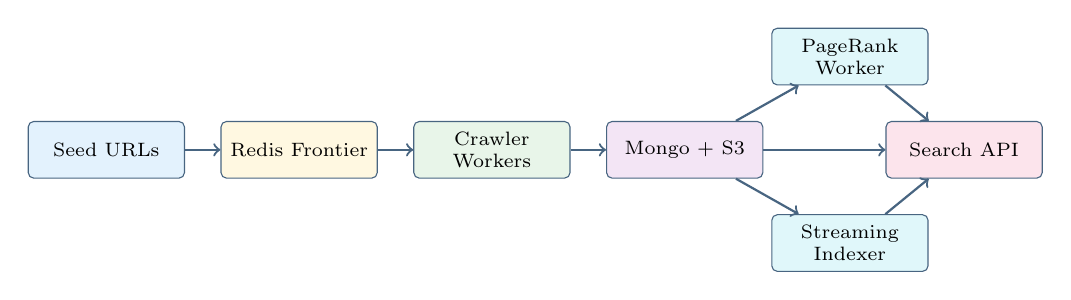
\begin{tikzpicture}[
      node distance=0.45cm,
      every node/.style={font=\scriptsize},
      box/.style={draw=Steel, rounded corners=2pt, minimum height=0.72cm, align=center, text width=1.75cm},
      arrow/.style={->, thick, draw=Steel}
    ]
    \node[box, fill=SoftBlue] (seed) {Seed URLs};
    \node[box, fill=SoftAmber, right=of seed] (redis) {Redis Frontier};
    \node[box, fill=SoftGreen, right=of redis] (worker) {Crawler Workers};
    \node[box, fill=SoftPurple, right=of worker] (storage) {Mongo + S3};
    \node[box, fill=SoftCyan, below right=0.45cm and 0.1cm of storage] (index) {Streaming Indexer};
    \node[box, fill=SoftCyan, above right=0.45cm and 0.1cm of storage] (pr) {PageRank Worker};
    \node[box, fill=SoftRose, right=1.55cm of storage] (api) {Search API};

    \draw[arrow] (seed) -- (redis);
    \draw[arrow] (redis) -- (worker);
    \draw[arrow] (worker) -- (storage);
    \draw[arrow] (storage) -- (index);
    \draw[arrow] (storage) -- (pr);
    \draw[arrow] (index) -- (api);
    \draw[arrow] (pr) -- (api);
    \draw[arrow] (storage) -- (api);
  \end{tikzpicture}

  \vspace{0.8em}
  \begin{block}{Flow summary}
    Seed URLs enter Redis. Workers fetch and parse pages. MongoDB commits page data and outbox events atomically. Streaming consumers update search and authority state. FastAPI serves ranked results.
  \end{block}
\end{frame}

\begin{frame}{System Architecture}
  \centering
  \includegraphics[width=\textwidth,height=0.78\textheight,keepaspectratio]{figures/architecture.pdf}

  \vspace{0.3em}
  \small Full architecture: Redis coordination, crawler workers, S3 (SeaweedFS) blob storage, MongoDB records, streaming consumers, and search API.
\end{frame}

\begin{frame}{Docker Compose Topology}
  \begin{columns}[T,totalwidth=\textwidth]
    \begin{column}{0.50\textwidth}
      \component{Docker Compose}
      {Runs Redis, MongoDB, the S3 store (SeaweedFS), crawler workers, streaming indexer, PageRank worker, search API, and seed helper as containers.}
      {It gives a reproducible setup where every service runs in an isolated container with the same network and environment.}
    \end{column}
    \begin{column}{0.46\textwidth}
      \begin{block}{What Docker gives us}
        \begin{itemize}
          \item Same setup for every evaluator machine.
          \item Easy service startup and shutdown.
          \item Multiple crawler workers can run side by side.
          \item Services communicate using Compose DNS names.
          \item CI runs the same Compose services.
        \end{itemize}
      \end{block}
    \end{column}
  \end{columns}
\end{frame}

\begin{frame}{Seed Helper}
  \component{Seed helper}
  {Reads \texttt{seed\_urls.txt} and inserts starting URLs into the Redis frontier.}
  {The crawler is pull-based. Workers need an initial frontier before they can start discovering more links.}

  \begin{block}{Role in the flow}
    The seed helper only starts the crawl. After that, crawler workers discover new links from downloaded pages and add those URLs back into Redis.
  \end{block}
\end{frame}

\begin{frame}{Redis: Coordination Layer}
  \begin{columns}[T,totalwidth=\textwidth]
    \begin{column}{0.52\textwidth}
      \component{Redis}
      {Stores the URL frontier, Bloom-filter dedupe bits, URL processing leases, domain locks, and robots/crawl-delay cache.}
      {Redis gives low-latency atomic coordination between many worker containers.}
    \end{column}
    \begin{column}{0.44\textwidth}
      \begin{block}{Key Redis structures}
        \begin{itemize}
          \item \texttt{crawler:active\_domains}
          \item \texttt{crawler:frontier:<domain>}
          \item \texttt{crawler:bloom}
          \item \texttt{crawler:processing}
          \item \texttt{lock:<domain>}
        \end{itemize}
      \end{block}
    \end{column}
  \end{columns}
\end{frame}

\begin{frame}{Crawler Worker}
  \begin{columns}[T,totalwidth=\textwidth]
    \begin{column}{0.50\textwidth}
      \component{crawler-worker}
      {Pulls URLs from Redis, checks politeness, downloads HTML, extracts clean text and outbound links, and writes page data to storage.}
      {It is autonomous and stateless except for shared Redis/Mongo/S3 state, so many workers can run at once.}
    \end{column}
    \begin{column}{0.46\textwidth}
      \begin{block}{Worker loop}
        \small
        \begin{enumerate}
          \item Claim URLs until 8 fetches are in flight, each on a domain whose lock it holds.
          \item Fetch on a thread pool; everything else stays on the main thread.
          \item Parse title, text, links.
          \item Save transaction + outbox events.
          \item Release URL lease after commit.
        \end{enumerate}
      \end{block}
    \end{column}
  \end{columns}
\end{frame}

\begin{frame}{Fetching: Failures, Size Cap, Shutdown}
  \begin{columns}[T,totalwidth=\textwidth]
    \begin{column}{0.48\textwidth}
      \begin{block}{Permanent vs.\ transient failures}
        \begin{itemize}
          \item 404/403/410, non-HTML, $>$5~MB: dropped at once.
          \item Timeouts, 5xx, 408, 429: retried with priority decay.
          \item Bodies are streamed under the cap, so one huge page cannot exhaust memory.
        \end{itemize}
      \end{block}
    \end{column}
    \begin{column}{0.48\textwidth}
      \begin{block}{Graceful shutdown}
        \begin{itemize}
          \item \texttt{docker stop} sends SIGTERM.
          \item The worker finishes in-flight fetches, flushes its batch, and releases its leases.
          \item Exit code 0 instead of 143; no pages lost.
        \end{itemize}
      \end{block}
    \end{column}
  \end{columns}
\end{frame}

\begin{frame}{Robots.txt And Politeness}
  \component{Robots and politeness}
  {Fetches \texttt{/robots.txt}, checks \texttt{can\_fetch}, caches robots content and crawl-delay in Redis, and enforces per-domain locks.}
  {Distributed crawlers must be polite. Multiple workers should not hit the same domain simultaneously.}

  \begin{block}{Policy}
    Every request identifies itself as \texttt{DistributedCrawler/1.0} with the repository URL, so site owners can recognise and target it in \texttt{robots.txt}. Disallowed URLs never enter the frontier. Each in-flight fetch holds its domain's lock, so concurrency never means two requests to one site.
  \end{block}
\end{frame}

\begin{frame}{S3 Blob Storage}
  \component{S3 store (SeaweedFS)}
  {Stores compressed raw HTML blobs in the shared \texttt{crawler-html} bucket. MongoDB stores only pointers and metadata.}
  {Large HTML blobs should not bloat MongoDB's working set. Shared object storage also works when workers and API run on different machines.}

  \begin{block}{Data split}
    MongoDB keeps searchable metadata and references; the S3 store keeps the heavier page payloads. The crawler speaks plain S3, so when MinIO stopped publishing images it was replaced by SeaweedFS with no code changes.
  \end{block}
\end{frame}

\begin{frame}{MongoDB Storage}
  \small
  \component{MongoDB}
  {Stores page metadata, clean text, content pointers, indexing state, graph edges, and PageRank scores.}
  {MongoDB gives durable structured storage and supports atomic updates across the crawler pipeline.}

  \begin{block}{Main collections}
    \begin{itemize}
      \item \texttt{pages\_metadata}
      \item \texttt{pages\_content}
      \item \texttt{pages\_documents}
      \item \texttt{index\_outbox}
      \item \texttt{graph\_outbox}
      \item \texttt{term\_postings}, \texttt{graph\_edges}, \texttt{pagerank\_nodes}
    \end{itemize}
  \end{block}
\end{frame}

\begin{frame}{Streaming Indexer}
  \component{streaming-indexer}
  {Consumes \texttt{index\_outbox}, loads clean text from \texttt{pages\_documents}, tokenizes/stems terms, computes term frequencies, and updates \texttt{term\_postings}.}
  {Indexing is moved out of crawler workers, so crawling stays fast and search state is updated asynchronously.}

  \begin{block}{Search index shape}
    \texttt{term\_postings} stores one document per \texttt{(term, url)} with term frequency, document length and a title flag --- everything BM25 needs, with no giant embedded posting arrays.
  \end{block}
\end{frame}

\begin{frame}{Incremental PageRank Worker}
  \component{pagerank-worker}
  {Consumes \texttt{graph\_outbox}, compares new outbound links with historical \texttt{graph\_edges}, applies PageRank contribution deltas, and pushes residuals through \texttt{pagerank\_nodes}.}
  {Authority scoring is expensive graph math; separating it from crawling keeps the crawler responsive.}

  \begin{block}{Local updates, same answer as a full recompute}
    Ranks use the unnormalized equation $x_v = (1-d) + d\sum_{u \to v} x_u / |N_u|$. A new page just starts with its own teleport mass, so no update ever touches the whole graph, and incremental ranks match a full power-iteration recompute (checked by a test).
  \end{block}
\end{frame}

\begin{frame}{Search API}
  \component{FastAPI search-api}
  {Tokenizes the query, scores matching \texttt{term\_postings} with BM25, takes the top candidates, joins \texttt{pagerank\_nodes}, and sorts and limits inside MongoDB.}
  {Search stays fast because it does not crawl, tokenize all documents, or recompute PageRank at query time.}

  \begin{block}{Ranking formula}
    \[
      \text{score} = \text{BM25}(q, u) \times \left(1 + 0.5 \ln\!\left(1 + \tfrac{\text{PageRank}(u)}{1-d}\right)\right)
    \]
    \small Title matches count 1.5$\times$; \texttt{mode=all} requires every query term.
  \end{block}
\end{frame}

\begin{frame}{Index And Search Flow}
  \centering
  \includegraphics[width=0.92\textwidth,height=0.62\textheight,keepaspectratio]{figures/index_search_flow.pdf}

  \begin{block}{Result}
    Crawled text becomes searchable postings, PageRank becomes authority, and the API combines both signals when answering a query.
  \end{block}
\end{frame}

\begin{frame}{Fault Tolerance}
  \begin{columns}[T,totalwidth=\textwidth]
    \begin{column}{0.50\textwidth}
      \begin{block}{Failures handled}
        \begin{itemize}
          \item Worker crashes mid-crawl.
          \item Worker stopped with \texttt{docker stop}.
          \item Duplicate URL discovery.
          \item Domain lock contention.
          \item Outbox consumer crash.
          \item PageRank transient write conflict.
        \end{itemize}
      \end{block}
    \end{column}
    \begin{column}{0.46\textwidth}
      \begin{block}{Mechanisms}
        \begin{itemize}
          \item Redis TTL leases.
          \item SIGTERM handler: drain and flush.
          \item Lua atomic frontier updates.
          \item MongoDB transactions.
          \item Outbox claim/reclaim.
          \item Transaction retry with backoff.
        \end{itemize}
      \end{block}
    \end{column}
  \end{columns}
\end{frame}

\begin{frame}{Results: Scaling}
  \begin{columns}[T,totalwidth=\textwidth]
    \begin{column}{0.49\textwidth}
      \centering
      \figureOrNote{figures/throughput_vs_workers.pdf}{0.98}

      \small Worker processes (1 fetch each)
    \end{column}
    \begin{column}{0.49\textwidth}
      \centering
      \figureOrNote{figures/throughput_vs_concurrency.pdf}{0.98}

      \small One worker, more in-flight fetches
    \end{column}
  \end{columns}
\end{frame}

\begin{frame}{Results: Search and Recovery}
  \begin{columns}[T,totalwidth=\textwidth]
    \begin{column}{0.49\textwidth}
      \centering
      \figureOrNote{figures/query_latency_by_type.pdf}{0.98}

      \small Search latency by query type
    \end{column}
    \begin{column}{0.49\textwidth}
      \centering
      \figureOrNote{figures/fault_tolerance_completed_pages.pdf}{0.98}

      \small One worker killed mid-crawl
    \end{column}
  \end{columns}
\end{frame}

\begin{frame}{Testing and CI}
  \begin{columns}[T,totalwidth=\textwidth]
    \begin{column}{0.48\textwidth}
      \begin{block}{Test suites}
        \begin{itemize}
          \item 25 unit tests, no infrastructure.
          \item PageRank: incremental vs.\ recompute on real MongoDB.
          \item Search: BM25 ranking behaviour end to end.
          \item Distributed test: 3 workers, one killed, search verified.
        \end{itemize}
      \end{block}
    \end{column}
    \begin{column}{0.48\textwidth}
      \begin{block}{GitHub Actions}
        \begin{itemize}
          \item \texttt{tests} job: all suites against the Compose MongoDB.
          \item \texttt{e2e} job: Redis + MongoDB + S3, then the distributed test.
          \item Database tests fail, not skip, if MongoDB is missing.
        \end{itemize}
      \end{block}
    \end{column}
  \end{columns}
\end{frame}

\begin{frame}{How One Page Moves Through The System}
  \begin{enumerate}
    \item A URL is selected from Redis according to priority and domain availability.
    \item A crawler worker checks robots.txt and takes the domain lock.
    \item The worker downloads HTML (alongside other domains' fetches), extracts text, and discovers outbound links.
    \item Raw HTML is compressed into the S3 store and page metadata is saved in MongoDB.
    \item Background workers update the search index and PageRank information.
    \item The Search API uses the prepared data to return ranked results quickly.
  \end{enumerate}
\end{frame}

\begin{frame}{Final System Summary}
  \centering
  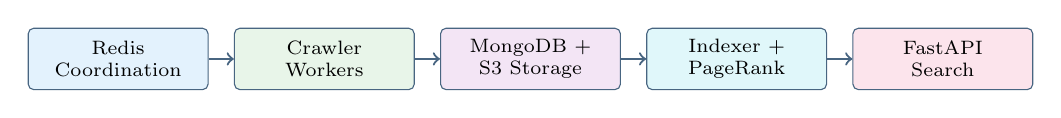
\begin{tikzpicture}[
      node distance=0.32cm,
      every node/.style={font=\scriptsize},
      box/.style={draw=Steel, rounded corners=2pt, minimum height=0.78cm, align=center, text width=2.05cm},
      arrow/.style={->, thick, draw=Steel}
    ]
    \node[box, fill=SoftBlue] (coord) {Redis\\Coordination};
    \node[box, fill=SoftGreen, right=of coord] (crawl) {Crawler\\Workers};
    \node[box, fill=SoftPurple, right=of crawl] (store) {MongoDB +\\S3 Storage};
    \node[box, fill=SoftCyan, right=of store] (process) {Indexer +\\PageRank};
    \node[box, fill=SoftRose, right=of process] (serve) {FastAPI\\Search};

    \draw[arrow] (coord) -- (crawl);
    \draw[arrow] (crawl) -- (store);
    \draw[arrow] (store) -- (process);
    \draw[arrow] (process) -- (serve);
  \end{tikzpicture}

  \vspace{1.0em}
  \begin{block}{Main contribution}
    The project connects distributed crawling, polite URL scheduling, durable storage, streaming indexing, graph-based authority scoring, and ranked search into one Dockerized pipeline.
  \end{block}
\end{frame}

\end{document}
